% ---------------- RELAZIONE PROGETTO DI PROGRAMMAZIONE AD OGGETTI (OOP) --------
\documentclass[a4paper,12pt]{report}

% ----------------------------- PREAMBLE --------------------------------------- 

\usepackage{alltt, fancyvrb, url}
\usepackage{graphicx}
\usepackage[utf8]{inputenc}
\usepackage{hyperref}

% Questo commentalo se vuoi scrivere in inglese.
\usepackage[italian]{babel}

\usepackage[italian]{cleveref}

\usepackage{comment}
\usepackage{microtype}
\usepackage{fancyhdr}

% hyperref settings
\hypersetup{
	colorlinks=true,
	linkcolor=black, %blue
	filecolor=magenta,      
	urlcolor=cyan,
	pdftitle={Sharelatex Example},
	bookmarks=true,
	pdfpagemode=FullScreen,
}

% ----------------------------- PREAMBLE END -----------------------------------

\title{Meta-relazione per\\``Programmazione ad Oggetti''}

\author{Danilo Pianini}
\date{\today}




\begin{document}

\maketitle

\tableofcontents

% \input: import the commands from filename.tex to target file.

% \include: does a \clearpage and does an \input.

% ============================ ABSTRACT =========================================

\begin{abstract}
	Questo documento è una relazione di meta livello, ossia una relazione che spiega come scrivere la relazione.
	%
	Lo scopo di questo documento è quello di aiutare gli studenti a comprendere quali punti trattare nella loro relazione, ed in che modo farlo, evitando di perdere del tempo prezioso in prolisse discussioni di aspetti marginali tralasciando invece aspetti di maggior rilievo.
	%
	Per ciascuna delle sezioni del documento sarà fornita una descrizione di ciò che ci si aspetta venga prodotto dal team di sviluppo, assieme ad un elenco (per forza di cose non esaustivo) di elementi che \emph{non} dovrebbero essere inclusi.
	
	Il modello della relazione segue il processo tradizionale di ingegneria del software fase per fase (in maniera ovviamente semplificata).
	%
	La struttura della relazione non è indicativa ma \textit{obbligatoria}.
	%
	Gli studenti dovranno produrre un documento che abbia la medesima struttura, non saranno accettati progetti la cui relazione non risponda al requisito suddetto.
	%
	Lo studente attento dovrebbe sforzarsi di seguire le tappe suggerite in questa relazione anche per l'effettivo sviluppo del progetto: oltre ad una considerevole semplificazione del processo di redazione di questo documento, infatti, il gruppo beneficerà di un processo di sviluppo più solido e collaudato, di tipo top-down.
	
	La meta-relazione verrà fornita corredata di un template \LaTeX{} per coloro che volessero cimentarsi nell'uso.
	%
	L'uso di \LaTeX{} è vantaggioso per chi ama l'approccio ``what you mean is what you get'', ossia voglia disaccoppiare il contenuto dall'effettivo rendering del documento, accollando al motore \LaTeX{} l'onere di produrre un documento gradevole con la struttura ed il contenuto forniti.
	%
	Chi non volesse installare l'ambiente di compilazione in locale può valutare l'utilizzo dell'applicazione web \href{https://www.overleaf.com/}{Overleaf}.
	%
	L'eventuale utilizzo di \LaTeX{} non è fra i requisiti, non è parte del corso di Programmazione ad Oggetti, e non sarà ovviamente valutato. I docenti accetteranno qualunque relazione in formato standard Portable Document Format (pdf), indipendentemente dal software con cui tale documento sarà redatto.
\end{abstract}

% ------------------------------------ ANALISI ----------------------------------

\chapter{Analisi}

\textsf{\small \textbf{Bullet Ballet} è un videogioco platform a scorrimento orizzontale, del genere \emph{Shoot 'em up} in 2D.}\\
\textsf{\small L'obiettivo del gioco è quello di realizzare più punti possibili per superare i propri record, in base alla distanza percorsa dal giocatore.}\\

\textsf{\small Ma non sarà tutto in discesa, il giocatore dovrà affrontare nemici con i più variegati equipaggiamenti, ostacoli di ogni sorta, varchi nella mappa e molto altro ancora..}\\
\textsf{\small Il giocatore potrà scegliere fra ben 8 mappe uniche e relative piattaforme in tema.}\\

\textsf{\small Inoltre, il giocatore potrà avvalersi a sua volta di effetti (bonus) sia positivi che negativi per poter sconfiggere le avversità che si presenteranno sul suo cammino.}\\

\textsf{\small Potrà, poi salvare tutti i suoi punteggi di gioco.}\\

\begin{comment}
In questo capitolo andrà fatta l'analisi dei requisiti e quella del problema, ossia verranno elencate le cose che l'applicazione dovrà fare (requisiti) e verrà descritto il dominio applicativo (analisi del problema).
%
In fase di analisi, è molto importante tenere a mente che non vi deve essere alcun riferimento al design né tantomeno alle tecnologie implementative, ovvero, non si deve indicare come il software sarà internamente realizzato.
%
La fase di analisi, infatti, \textit{precede} qualunque azione di design o di implementazione.
\end{comment}

\section{Requisiti}

\textsf{\small L'applicazione mostra, all'avvio, un menù di gioco con le seguenti voci: \emph{New Game}, \emph{Load Game}, \emph{Settings},\emph{Quit}.}\\

\begin{comment}
Nell'analisi dei \emph{requisiti} dell'applicazione si dovrà spiegare cosa l'applicazione dovrà fare.
%
Non ci si deve concentrare sui particolari problemi, ma esclusivamente su cosa si desidera che l'applicazione faccia.
%
È consigliato descrivere separatamente i requisiti funzionali (quelli che descrivono l'effettivo
comportamento dell'applicazione) da quelli non funzionali (requisiti che non riguardano direttamente
aspetti comportamentali, come sicurezza, performance, eccetera).
\end{comment}

\begin{comment}
\subsection*{Elementi positivi}
\begin{itemize}
	\item Si fornisce una descrizione in linguaggio naturale di ciò che il software dovrà fare.
	\item Gli obiettivi sono spiegati con chiarezza, per punti.
	\item Se il software è stato commissionato o è destinato ad un utente o compagnia specifici, il committente viene nominato.
	\item Se vi sono termini il cui significato non è immediatamente intuibile, essi vengono spiegati.
	\item Vengono descritti separatamente requisiti funzionali e non funzionali.
	\item Considerato a un paio di pagine un limite ragionevole alla lunghezza della parte sui requisiti, in quello spazio si deve cercare di chiarire \textit{tutti} gli aspetti dell'applicazione, non lasciando decisioni che impattano la parte ``esterna'' alla discussione del design (che dovrebbe solo occuparsi della parte ``interna'').
\end{itemize}

\subsection*{Elementi negativi}
\begin{itemize}
	\item Si forniscono indicazioni circa le soluzioni che si vogliono adottare
	\item Si forniscono dettagli di tipo tecnico o implementativo (parlando di classi, linguaggi di programmazione, librerie, eccetera)
\end{itemize}

\subsection*{Esempio}
Il software, commissionato dal gestore del centro di ricerca ``Aperture Laboratories Inc.''\footnote{\url{http://aperturescience.com/}}, mira alla costruzione di una intelligenza artificiale di nome GLaDOS (Genetic Lifeform and Disk Operating System).
%
Per intelligenza artificiale si intende un software in grado di assumere decisioni complesse in maniera semi autonoma sugli argomenti di sua competenza, a partire dai vincoli e dagli obiettivi datigli dall'utente.
\end{comment}

\subsubsection{Requisiti funzionali}

\begin{itemize}
	\item \textsf{\small \emph{Mappa scorrevole}: Il giocatore potrà muoversi in una mappa a scorrimento orizzontale con uno sfondo statico.}
	\item \textsf{\small \emph{Menù di gioco}: Non appena lanciata l'applicazione, l'utente vedrà un menù di gioco con diverse opzioni tra cui potrà scegliere.}
	\item \textsf{\small \emph{Menù di pausa}: Il giocatore potrà mettere il gioco in pausa attraverso un dato pulsante della tastiera, scelto nelle impostazioni.}
	\item \textsf{\small \emph{Personaggio}: Il giocatore potrà scegliere un personaggio e muoverlo in partita.}
	\item \textsf{\small \emph{Nemici}: Verranno generati diversi nemici che il giocatore dovrà affrontare.}
	\item \textsf{\small \emph{Ostacoli e oggetti raccoglibili}: Verranno creati nella mappa degli ostacoli che bloccheranno la strada e degli oggetti che il giocatore potrà raccogliere per ricevere un (power up) bonus od un malus.}
	\item \textsf{\small \emph{Salvataggio del punteggio e classifica}: Terminata la partita, il punteggio di gioco potrà essere salvato e verrà generata una classifica finale.}
	\item \textsf{\small \emph{Suoni ed effetti sonori}: La durata della partita verrà accompagnata da una colonna sonora e agli effetti sonori prodotti dall'environment di gioco.}
	\item \textsf{\small \emph{Fisica di gioco}: Tutti le entità di gioco saranno dotati di una fisica ed una gravità propria.}
	%\item \textsf{\small }
	%\item \textsf{\small }
	%\item \textsf{\small }
	%\item \textsf{\small }
\end{itemize}

\begin{comment}
\begin{itemize}
\item La suddetta intelligenza artificiale dovrà occuparsi di coordinare le attività all'interno
delle camere di test di Aperture, guidando l'utente attraverso un certo numero di sfide di
difficoltà crescente. Una camera di test è un ambiente realizzato da Aperture Laboratories Inc. al
fine di mettere alla prova le proprie tecnologie di manipolazione dell'ambiente. All'interno della
camera di test, un soggetto qualificato è incaricato di sfruttare gli strumenti messi a
disposizione da Aperture per risolvere alcuni rompicapi. I rompicapi sono di tipo fisico (ad
esempio, manipolazione di oggetti, pressione di pulsanti, azionamento di leve), e si ritengono
conclusi una volta che il soggetto riesce a trovare l'uscita dalla camera di test.
\item Il piano preciso ed il numero delle sfide sarà variabile, e GLaDOS dovrà essere in grado di adattarsi dinamicamente e di fornire indicazioni di guida.
\item La personalità di GLaDOS dovrà essere modificabile.
\item GLaDOS dovrà essere in grado di comunicare col reparto cucina di Aperture, per ordinare torte da donare agli utenti che completassero l'ultima camera di test con successo.
\end{itemize}
\end{comment}

%\subsubsection{Requisiti non funzionali}
\subsection{Requisiti opzionali}

\textsf{\small Questi requisiti non concorrono a far parte delle funzionalità minime del gioco e per questioni di tempistica e/o di budget non verranno necessariamente implementate.}\\

\begin{itemize}
	\item \textsf{\small \emph{Oggetti dinamici}: ovvero oggetti che si muovono e che hanno una animazione.}
	\item \textsf{\small \emph{Market}: per poter comprare/vendere skin (mimetiche) di gioco con valuta reale o in gioco. (o fittizia del gioco)}
	\item \textsf{\small \emph{Modalità storia}: una modalità con una storia di gioco e diversi livelli che il giocatore dovrà sbloccare per poter continuare ad avanzare nel gioco.}
	\item \textsf{\small \emph{Statistiche di gioco}: Varie statistiche di gioco, mostrate in diversi diagrammi.}
	\item \textsf{\small \emph{Difficoltà di gioco}: Possibilità di scegliere diverse difficoltà che potrebbero aggiungere numero di nemici/ostacoli/oggetti di varia natura e/o incrementare la loro vita.}
	%\item \textsf{\small }
\end{itemize}

\begin{comment}
\begin{itemize}
\item GLaDOS dovrà essere estremamente efficiente nell'uso delle risorse. Le specifiche tecniche parlano della possibilità di funzionare su dispositivi alimentati da una batteria a patata.
\end{itemize}
\end{comment}

\section{Analisi e modello del dominio}

\textsf{\small L'applicazione fornisce un giocatore che tramite input dell'utente può essere spostato a destra, a sinistra e farlo saltare. Il quale, potrà interagire con le varie entità, sia statiche che dinamiche del gioco, quali \emph{nemici}, \emph{armi}, \emph{monete}, \emph{items}, \emph{ostacoli}.
Ognuna di queste entità interagirà in maniere differenti col player: }\\

\begin{itemize}
	\item \textsf{\small \emph{Enemy}, ostacolerà il player a colpi di mitra.} %TODO: da modificare.
	\item \textsf{\small \emph{Item}, una volta raccolta dal player, gli fornirà o un \textbf{bonus}, come una vita extra oppure un \textbf{malus} come un effetto di volevo per tot tempo.}
	\item \textsf{\small \emph{monete}, faranno aumentare il punteggio e il numero di monete del gioco da usare nel mercato per poter comprare nuove skins, in game-items, ecc..}
	\item \textsf{\small \emph{Armi}, dopo essere state raccolte verranno equipaggiate al giocatore.}
	\item \textsf{\small \emph{Ostacoli}, se il player ci colliderà, subirà del danno.}
\end{itemize}

\textsf{\small Il gioco si conclude quando e se il player riesce a raggiungere la fine della mappa senza morire.}
\textsf{\small Se il player viene ucciso prima di raggiungere la fine, allora viene eliminato e la partita è persa.}\\

\textsf{\small Ogni round è a sè stante, finita la partita, al player verrà assegnato un punteggio e potrà scegliere se rigiocare od uscire.}\\

%TODO: aggiungere UML.

%\begin{landscape}
	\begin{figure}[h]
		\centering{}
		%\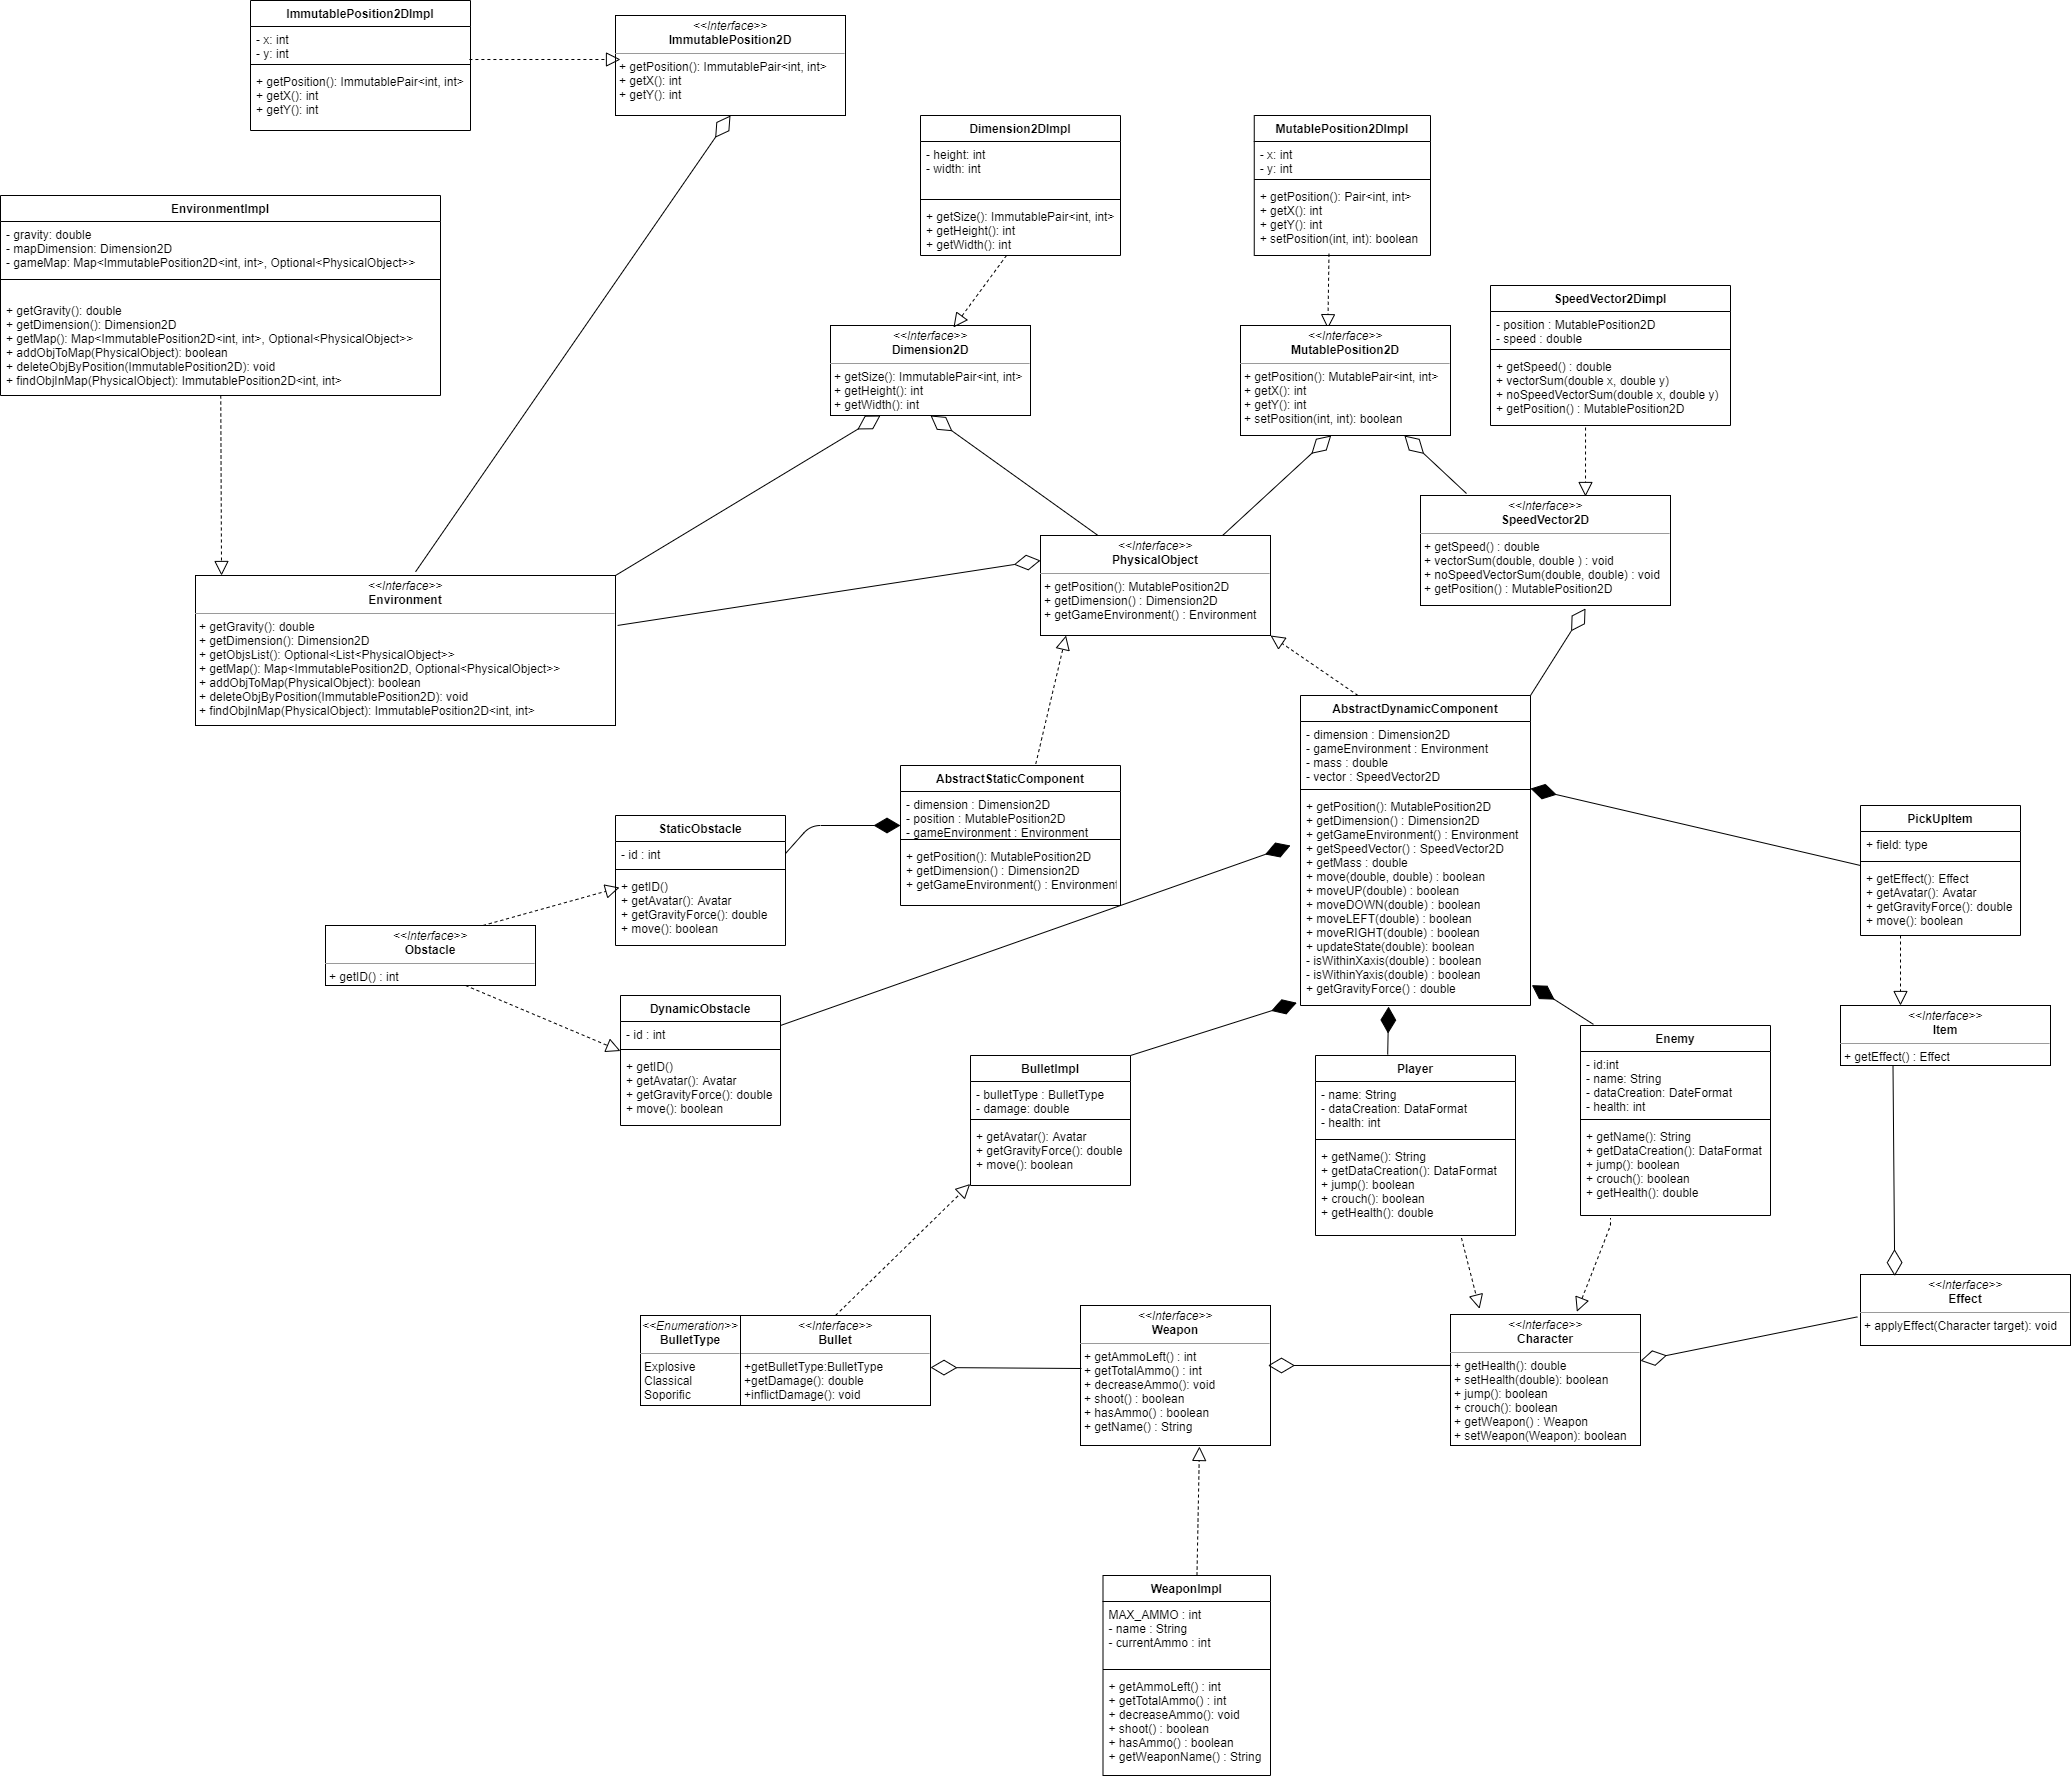
\includegraphics[width=1.2\linewidth]{./img/model.png} %TODO: cambiare UML
		\caption{Schema UML dell'analisi del problema, con rappresentate le entità principali ed i rapporti fra loro.}
		\label{img:analysis}
	\end{figure}
%\end{landscape}

\begin{comment}

In questa sezione si descrive il modello del \textit{dominio
	applicativo}, descrivendo le \textit{entità} in gioco ed i rapporti fra loro.
%
Si possono sollevare eventuali aspetti particolarmente impegnativi, descrivendo perché lo sono, senza inserire idee circa possibili soluzioni, ovvero sull'organizzazione interna del software.
%
Infatti, la fase di analisi va effettuata \textbf{prima} del progetto: né il progetto né il software esistono nel momento in cui si effettua l'analisi.
%
La discussione di aspetti propri del software (ossia, della \textit{soluzione} al problema e non del problema stesso) appartengono alla sfera della progettazione, e vanno discussi successivamente.

È obbligatorio fornire uno schema UML del dominio, che diventerà anche lo scheletro della
parte ``entity'' del modello dell'applicazione, ovvero degli elementi costitutivi del modello (in ottica MVC - Model View Controller): se l'analisi è ben fatta, dovreste ottenere una gerarchia di concetti che rappresentano le entità che compongono il problema da risolvere.
%
Un'analisi ben svolta \textbf{prima} di cimentarsi con lo sviluppo rappresenta un notevole aiuto per
le fasi successive: è sufficiente descrivere a parole il dominio, quindi estrarre i sostantivi
utilizzati, capire il loro ruolo all'interno del problema, le relazioni che intercorrono fra loro, e
reificarli in interfacce.

\subsection*{Elementi positivi}
\begin{itemize}
	\item Viene descritto accuratamente il modello del dominio.
	\item Alcuni problemi, se non risolubili in assoluto o nel monte ore, vengono dichiarati come problemi che non saranno risolti o sarano risolti in futuro.
	\item Si modella il dominio in forma di UML, descrivendolo appropriatamente.
\end{itemize}

\subsection*{Elementi negativi}
\begin{itemize}
	\item Manca una descrizione a parole del modello del dominio.
	\item Manca una descrizione UML delle entità del dominio e delle relazioni che intercorrono fra loro.
	\item Vengono elencate soluzioni ai problemi, invece della descrizione degli stessi.
	\item Vengono presentati elementi di design, o peggio aspetti implementativi.
	\item Viene mostrato uno schema UML che include elementi implementativi o non utili alla descrizione del dominio, ma volti alla soluzione (non devono vedersi, ad esempio, campi o metodi privati, o cose che non siano equivalenti ad interfacce).
\end{itemize}

\subsection*{Esempio}
GLaDOS dovrà essere in grado di accedere ad un'insieme di camere di test.
%
Tale insieme di camere prende il nome di percorso.
%
Ciascuna camera è composta di challenge successivi.
%
GLaDOS è responsabile di associare a ciascun challenge un insieme di consigli (suggestions) destinati all'utente (subject), dipendenti da possibili eventi.
%
GLaDOS dovrà poter comunicare coi locali cucina per approntare le torte.
%
Le torte potranno essere dolci, oppure semplici promesse di dolci che verranno disattese.

Gli elementi costitutivi il problema sono sintetizzati in \Cref{img:analysis}.

La difficoltà primaria sarà quella di riuscire a correlare lo stato corrente dell'utente e gli eventi in modo tale da generare i corretti suggerimenti.
%
Questo richiederà di mettere in campo appropriate strategie di intelligenza artificiale.

Data la complessità di elaborare consigli via AI senza intervento umano, la prima versione del software fornita prevederà una serie di consigli forniti dall'utente.

Il requisito non funzionale riguardante il consumo energetico richiederà studi specifici sulle performance di GLaDOS che non potranno essere effettuati all'interno del monte ore previsto: tale feature sarà oggetto di futuri lavori.

\begin{figure}[h]
	\centering{}
	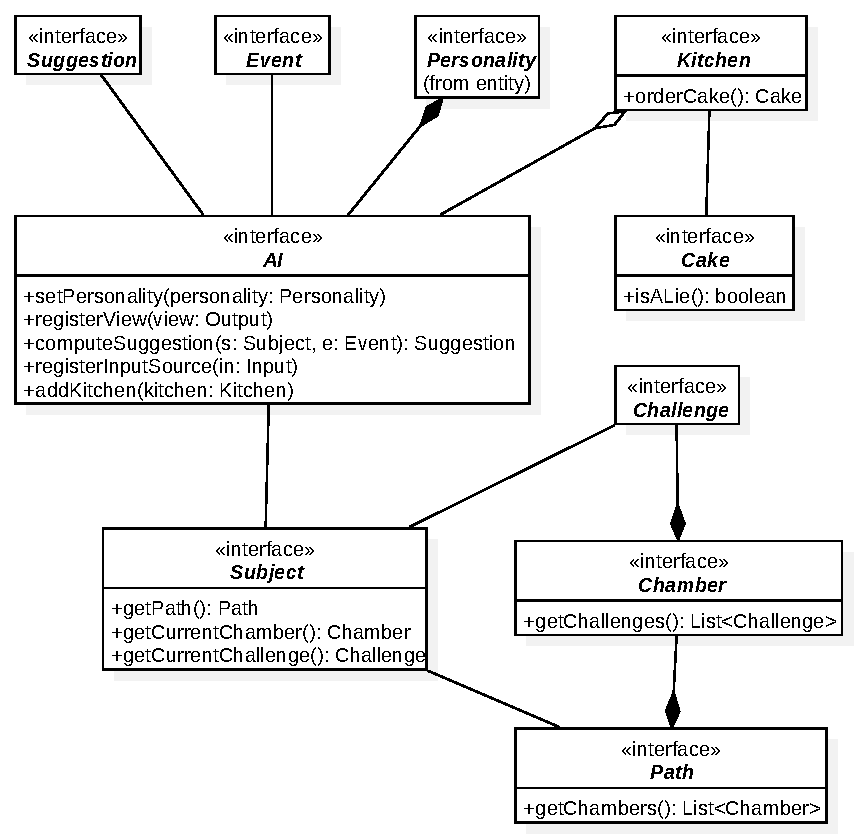
\includegraphics{img/analysis.pdf}
	\caption{Schema UML dell'analisi del problema, con rappresentate le entità principali ed i rapporti fra loro}
	\label{img:analysis}
\end{figure}

\end{comment}

% ---------------------------------- DESIGN -------------------------------------

\chapter{Design}

\begin{comment}
In questo capitolo si spiegano le strategie messe in campo per realizzare la soluzione ai problemi identificati nell'analisi.

Si parte da una visione architetturale, il cui scopo è informare il lettore di quale sia il funzionamento dell'applicativo realizzato ad alto livello.
%
In particolare, è necessario descrivere accuratamente in che modo i componenti principali del sistema si coordinano fra loro.
%
A seguire, si dettagliano alcune parti del design, quelle maggiormente rilevanti al fine di chiarificare la logica con cui sono stati risolti i problemi dell'applicazione.
\end{comment}

\section{Architettura}

\textsf{\small L'obiettivo del team era quello di poter lavorare ognuno alla propria parte indipendentemente ed evitando conflitti, per poi poterle collegare tutte assieme alla fine.}\\

\textsf{\small Il progetto sfrutta quindi il pattern architetturale \textbf{MVC} (\emph{M}odel \emph{V}iew \emph{C}ontroller) che permette di suddividere la gestione dell'applicativo in tre parti separate: }\\

\begin{itemize} %TODO: ingrandire questa parte oppure scrivere di più nell'introduzione del Design.
	\item \textsf{\small \textbf{Model}: dove vengono effettivamente modellate le entità di gioco. In questa parte vengono gestiti tutti gli aspetti riguardanti la logica, la gestione, la fisica, le caratteristiche e il comportamento delle componenti di gioco.}
	%si occupa dell'interfaccia grafica
	\item \textsf{\small \textbf{View}: si occupa degli aspetti grafici, quali esporre le effettive entità del \emph{Model} sullo schermo di gioco. La \emph{View} comprende anche il menù di gioco e la schermata di fine partita per esaminare i risultati della classifica. Riguarda, inoltre, anche la parte di generazione delle mappa che comprende vari tipi di sfondi e relative piattaforme in tema, monete, oggetti, armi e nemici.}
	% Inoltre, riguarda anche
	\item \textsf{\small \textbf{Controller}: è il concreto ponte, tra il \emph{Model} e la \emph{View}, consente di collegare la parte logica con quella visiva. La sua funzione è quella di ricevere input della tastiera dall'utente, inviarlo al \emph{Model} per essere elaborato e alla \emph{View} per avere un riscontro visivo.}
\end{itemize}

\textsf{\small Di seguito, un UML riguardante il pattern architetturale \textbf{MVC} utilizzato:}\\

\begin{figure}[htp]
	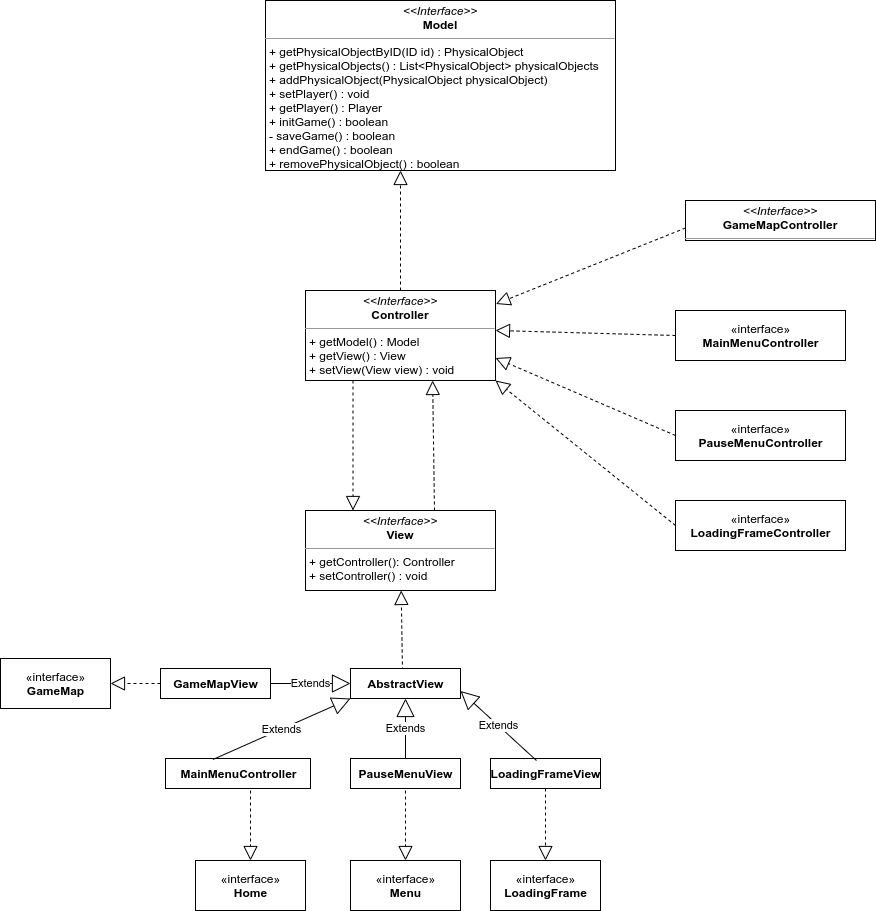
\includegraphics[width=1.2\linewidth]{./img/mvc.png}
	\caption{Schema UML del pattern architetturale MVC.}
	\label{img:mvc}
\end{figure}

%\newpage

\begin{comment}

Questa sezione spiega come le componenti principali del software interagiscono fra loro.
%
In particolare, qui va spiegato \textbf{se} e \textbf{come} è stato utilizzato il pattern
architetturale model-view-controller (e/o alcune sue declinazioni specifiche, come entity-control-boundary).

Se non è stato utilizzato MVC, va spiegata in maniera molto accurata l'architettura scelta, giustificandola in modo appropriato.

Se è stato scelto MVC, vanno identificate con precisione le interfacce e classi che rappresentano i punti d'ingresso per modello, view, e controller.
Raccomandiamo di sfruttare la definizione del dominio fatta in fase di analisi per capire quale sia l'entry point del model, e di non realizzare un'unica macro-interfaccia che, spesso, finisce con l'essere il prodromo ad una ``God class''.
%
Consigliamo anche di separare bene controller e model, facendo attenzione a non includere nel secondo strategie d'uso che appartengono al primo.

In questa sezione vanno descritte, per ciascun componente architetturale che ruoli ricopre (due o tre ruoli al massimo), ed in che modo interagisce (ossia, scambia informazioni) con gli altri componenti dell'architettura.
%
Raccomandiamo di porre particolare attenzione al design dell'interazione fra view e controller: se ben progettato, sostituire in blocco la view non dovrebbe causare alcuna modifica nel controller (tantomeno nel model).

\subsection*{Elementi positivi}
\begin{itemize}
	\item Si mostrano pochi, mirati schemi UML dai quali si deduce con chiarezza quali sono le parti principali del software e come interagiscono fra loro.
	\item Si mette in evidenza se e come il pattern architetturale model-view-controller è stato applicato, anche con l'uso di un UML che mostri le interfacce principali ed i rapporti fra loro.
	\item Si discute se sia semplice o meno, con l'architettura scelta, sostituire in blocco la view: in un MVC ben fatto, controller e modello non dovrebbero in alcun modo cambiare se si transitasse da una libreria grafica ad un'altra (ad esempio, da Swing a JavaFX, o viceversa).
\end{itemize}

\subsection*{Elementi negativi}
\begin{itemize}
	\item L'architettura è fatta in modo che sia impossibile riusare il modello per un software diverso che affronta lo stesso problema.
	\item L'architettura è tale che l'aggiunta di una funzionalità sul controller impatta pesantemente su view e/o modello.
	\item L'architettura è tale che la sostituzione in blocco della view impatta sul controller o, peggio ancora, sul modello.
	\item Si presentano UML caotici, difficili da leggere.
	\item Si presentano UML in cui sono mostrati elementi di dettaglio non appartenenti all'architettura, ad esempio includenti campi o con metodi che non interessano la parte di interazione fra le componenti principali del software.
	\item Si presentano schemi UML con classi (nel senso UML del termine) che ``galleggiano'' nello schema, non connesse, ossia senza relazioni con il resto degli elementi inseriti.
	\item Si presentano elementi di design di dettaglio, ad esempio tutte le classi e interfacce del modello o della view.
	\item Si discutono aspetti implementativi, ad esempio eventuali librerie usate oppure dettagli di codice.
\end{itemize}

\subsection*{Esempio}

L'architettura di GLaDOS segue il pattern architetturale MVC.
%
Più nello specifico, a livello architetturale, si è scelto di utilizzare MVC in forma ``ECB'', ossia ``entity-control-boundary''\footnote{
	Si fa presente che il pattern ECB effettivamente esiste in letteratura come ``istanza'' di MVC, e chi volesse può utilizzarlo come reificazione di MVC.
}.
%
GLaDOS implementa l'interfaccia AI, ed è il controller del sistema.
Essendo una intelligenza artificiale, è una classe attiva.
%
GLaDOS accetta la registrazione di Input ed Output, che fanno parte della ``view'' di MVC, e sono il ``boundary'' di ECB.
Gli Input rappresentano delle nuove informazioni che vengono fornite all'IA, ad esempio delle modifiche nel valore di un sensore, oppure un comando da parte dell'operatore.
Questi input infatti forniscono eventi.
Ottenere un evento è un'operazione bloccante: chi la esegue resta in attesa di un effettivo evento.
Di fatto, quindi, GLaDOS si configura come entità \textit{reattiva}.
Ogni volta che c'è un cambio alla situazione del soggetto, GLaDOS notifica i suoi Output,
informandoli su quale sia la situazione corrente.
%
Conseguentemente, GLaDOS è un ``observable'' per Output.

\begin{figure}[h]
	\centering{}
	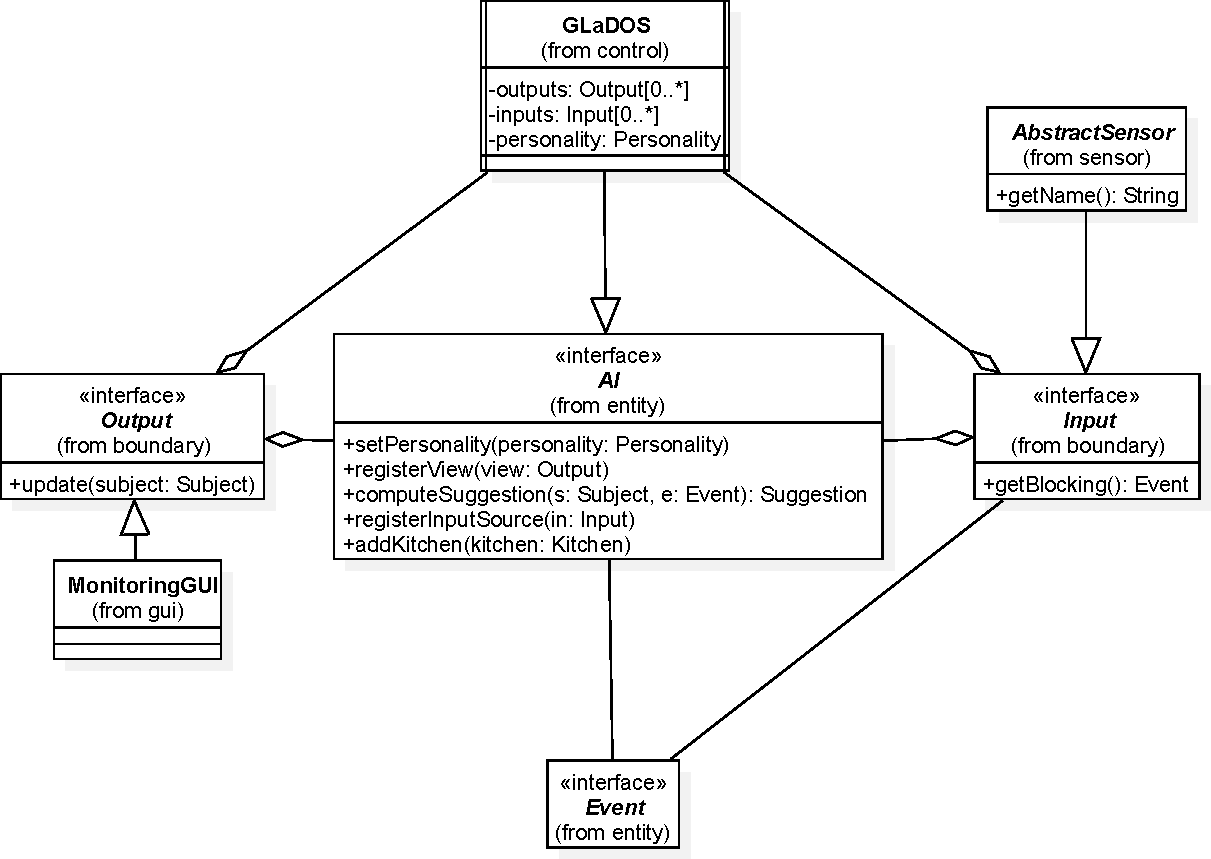
\includegraphics[width=\textwidth]{img/arch}
	\caption{Schema UML architetturale di GLaDOS. L'interfaccia \texttt{GLaDOS} è il controller del sistema, mentre \texttt{Input} ed \texttt{Output} sono le interfacce che mappano la view (o, più correttamente in questo specifico esempio, il boundary). Un'eventuale interfaccia grafica interattiva dovrà implementarle entrambe.}
	\label{img:goodarch}
\end{figure}

Con questa architettura, possono essere aggiunti un numero arbitrario di input ed output
all'intelligenza artificiale.
%
Ovviamente, mentre l'aggiunta di output è semplice e non richiede alcuna modifica all'IA, la
presenza di nuovi tipi di evento richiede invece in potenza aggiunte o rifiniture a GLaDOS.
%
Questo è dovuto al fatto che nuovi Input rappresentano di fatto nuovi elementi della business
logic, la cui alterazione od espansione inevitabilmente impatta il controller del progetto.

In \Cref{img:goodarch} è esemplificato il diagramma UML architetturale.

\end{comment}

\section{Design dettagliato}

%TODO: commentare questa parte del prof. quando avremo tutti finito di scrivere la nostra. -----------------  INIZIO -----------------------------------

In questa sezione si possono approfondire alcuni elementi del design con maggior dettaglio.
%
Mentre ci attendiamo principalmente (o solo) interfacce negli schemi UML delle sezioni precedenti, in questa sezione è necessario scendere in maggior dettaglio presentando la struttura di alcune sottoparti rilevanti dell'applicazione.
%
È molto importante che, descrivendo un problema, quando possibile si mostri che non si è re-inventata la ruota ma si è applicato un design pattern noto.
%
È assolutamente inutile, ed è anzi controproducente, descrivere classe-per-classe (o peggio ancora metodo-per-metodo) com'è fatto il vostro software: è un livello di dettaglio proprio della documentazione dell'API (deducibile dalla Javadoc).

\textbf{È necessario che ciascun membro del gruppo abbia una propria sezione di design dettagliato,
	di cui sarà il solo responsabile}.
%
Ciascun autore dovrà spiegare in modo corretto e giustamente approfondito (non troppo in dettaglio, non superficialmente) il proprio contributo.
%
È importante focalizzarsi sulle scelte che hanno un impatto positivo sul riuso, sull'estensibilità, e sulla chiarezza dell'applicazione.
%
Esattamente come nessun ingegnere meccanico presenta un solo foglio con l'intero progetto di una vettura di Formula 1, ma molteplici fogli di progetto che mostrano a livelli di dettaglio differenti le varie parti della vettura e le modalità di connessione fra le parti, così ci aspettiamo che voi, futuri ingegneri informatici, ci presentiate prima una visione globale del progetto, e via via siate in grado di dettagliare le singole parti, scartando i componenti che non interessano quella in esame.
%
Per continuare il parallelo con la vettura di Formula 1, se nei fogli di progetto che mostrano il
design delle sospensioni anteriori appaiono pezzi che appartengono al volante o al turbo, c'è una
chiara indicazione di qualche problema di design.

Usare correttamente i design pattern in questa sezione è molto importante: se vengono utilizzati correttamente, è molto probabile riuscire a progettare il software in modo corretto, estensibile, e riusabile.
%
Per ogni pattern utilizzato si presenti:
\begin{itemize}
	\item almeno un paragrafo che spieghi come è reificato nel progetto (ad esempio: nel caso di Template Method, qual è il metodo template; nel caso di Strategy, quale interfaccia del progetto rappresenta la strategia, e quali sono le sue implementazioni; nel caso di Decorator, qual è la classe astratta che fa da Decorator e quali sono le sue implementazioni concrete; eccetera);
	\item almeno uno schema UML che grafichi quanto sopra descritto.
\end{itemize}
%
La presenza di pattern di progettazione \emph{correttamente utilizzati} è valutata molto positivamente.
%
L'uso inappropriato è invece valutato negativamente: a tal proposito, si raccomanda di porre particolare attenzione all'abuso di Singleton, che, se usato in modo inappropriato, è di fatto un anti-pattern.

\subsection*{Elementi positivi}

\begin{itemize}
	\item Ogni membro del gruppo discute le proprie decisioni di progettazione, ed in particolare le azioni volte ad anticipare possibili cambiamenti futuri (ad esempio l'aggiunta di una nuova funzionalità, o il miglioramento di una esistente).
	\item Si identificano, utilizzano \textit{appropriatamente}, e descrivono come suggerito diversi design pattern.
	\item Ogni membro del gruppo identifica i pattern utilizzati nella sua sottoparte.
	\item Si mostrano gli aspetti di design più rilevanti dell'applicazione, mettendo in luce la maniera in cui si è costruita la soluzione ai problemi descritti nell'analisi.
	\item Si tralasciano aspetti strettamente implementativi e quelli non rilevanti, non mostrandoli negli schemi UML (ad esempio, campi privati) e non descrivendoli.
	\item Si mostrano le principali interazioni fra le varie componenti che collaborano alla soluzione di un determinato problema.
	\item Ciascun design pattern identificato presenta una piccola descrizione del problema calato
	nell'applicazione, uno schema UML che ne mostra la concretizzazione nelle classi del progetto, ed
	una breve descrizione della motivazione per cui tale pattern è stato scelto. Ad esempio, se si
	dichiara di aver usato Observer, è necessario specificare chi sia l'observable e chi l'observer; se
	si usa Template Method, è necessario indicare quale sia il metodo template; se si usa Strategy, è
	necessario identificare l'interfaccia che rappresenta la strategia; e via dicendo.
\end{itemize}

\subsection*{Elementi negativi}
\begin{itemize}
	\item Il design del modello risulta scorrelato dal problema descritto in analisi.
	\item Si tratta in modo prolisso, classe per classe, il software realizzato.
	\item Non si presentano schemi UML esemplificativi.
	\item Non si individuano design pattern, o si individuano in modo errato (si spaccia per design pattern qualcosa che non lo è).
	\item Si utilizzano design pattern in modo inopportuno. Un esempio classico è l'abuso di
	Singleton per entità che possono essere univoche ma non devono necessariamente esserlo. Si rammenta
	che Singleton ha senso nel secondo caso (ad esempio \texttt{System} e \texttt{Runtime} sono
	singleton), mentre rischia di essere un problema nel secondo. Ad esempio, se si rendesse singleton
	il motore di un videogioco, sarebbe impossibile riusarlo per costruire un server per partite online
	(dove, presumibilmente, si gestiscono parallelamente più partite).
	\item Si producono schemi UML caotici e difficili da leggere, che comprendono inutili elementi
	di dettaglio.
	\item Si presentano schemi UML con classi (nel senso UML del termine) che ``galleggiano'' nello schema, non connesse, ossia senza relazioni con il resto degli elementi inseriti.
	\item Si tratta in modo inutilmente prolisso la divisione in package, elencando ad esempio le classi una per una.
\end{itemize}

\subsection*{Esempio minimale (e quindi parziale) di sezione di progetto con UML ben realizzati}

In questa sezione ci si concentrerà sugli aspetti di personalità e sul funzionamento del reporting di GLaDOS.

Il sistema per la gestione della personalità utilizza il pattern Strategy, come da
\Cref{img:strategy}: le implementazioni di \texttt{Personality} possono essere modificate, e la
modifica impatta direttamente sul comportamento di GLaDOS.

\begin{figure}[h]
	\centering{}
	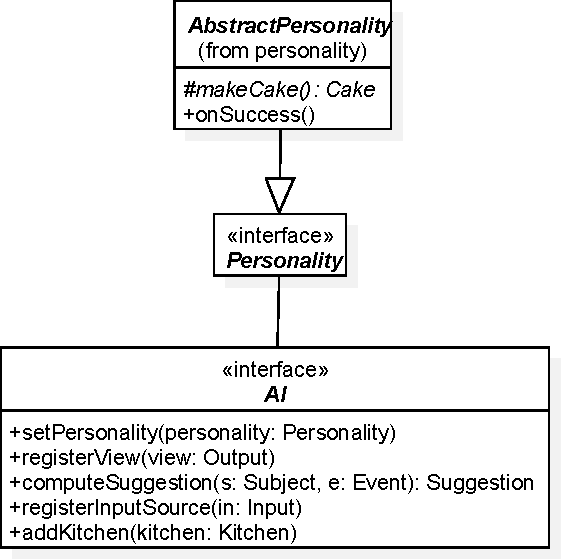
\includegraphics[width=\textwidth]{img/strategy}
	\caption{Rappresentazione UML del pattern Strategy per la personalità di GLaDOS}
	\label{img:strategy}
\end{figure}

\begin{figure}[h]
	\centering{}
	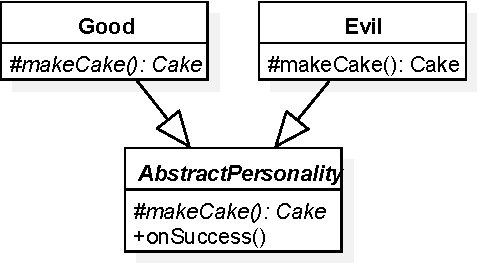
\includegraphics[width=\textwidth]{img/template}
	\caption{Rappresentazione UML dell'applicazione del pattern Template Method alla gerarchia delle Personalità}
	\label{img:template}
\end{figure}

Sono state attualmente implementate due personalità, una buona ed una cattiva.
Quella buona restituisce sempre una torta vera, mentre quella cattiva restituisce sempre la
promessa di una torta che verrà in realtà disattesa.
Dato che le due personalità differiscono solo per il comportamento da effettuarsi in caso di percorso completato con successo, è stato utilizzato il pattern template method per massimizzare il riuso, come da \Cref{img:template}.
Il metodo template è \texttt{onSuccess()}, che chiama un metodo astratto e protetto
\texttt{makeCake()}.

\begin{figure}[h]
	\centering{}
	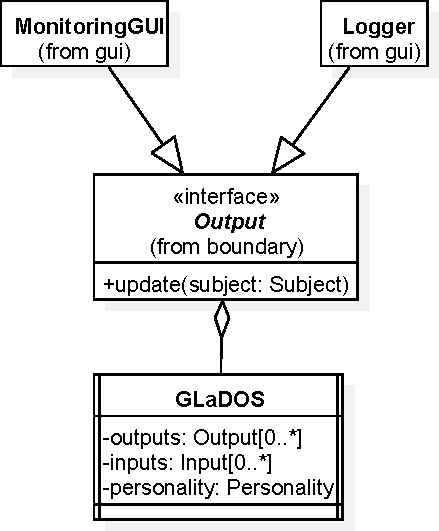
\includegraphics[width=.7\textwidth]{img/observer}
	\caption{Il pattern Observer è usato per consentire a GLaDOS di informare tutti i sistemi di output in ascolto}
	\label{img:observer}
\end{figure}

Per quanto riguarda il reporting, è stato utilizzato il pattern Observer per consentire la
comunicazione uno-a-molti fra \texttt{GLaDOS} ed i sistemi di output.
%
\texttt{GLaDOS} è observable, e le istanze di \texttt{Input} sono observer.
%
Il suo utilizzo è esemplificato in \Cref{img:observer}

\subsection*{Contro-esempio: pessimo diagramma UML}

In \Cref{img:badarch} è mostrato il modo \textbf{sbagliato} di fare le cose.
%
Questo schema è fatto male perché:
\begin{itemize}
	\item È caotico.
	\item È difficile da leggere e capire.
	\item Vi sono troppe classi, e non si capisce bene quali siano i rapporti che intercorrono fra loro.
	\item Si mostrano elementi implementativi irrilevanti, come i campi e i metodi privati nella classe \texttt{AbstractEnvironment}.
	\item Se l'intenzione era quella di costruire un diagramma architetturale, allora lo schema è ancora più sbagliato, perché mostra pezzi di implementazione.
	\item Una delle classi, in alto al centro, galleggia nello schema, non connessa a nessuna altra classe, e di fatto costituisce da sola un secondo schema UML scorrelato al resto
	\item Le interfacce presentano tutti i metodi e non una selezione che aiuti il lettore a capire quale parte del sistema si vuol mostrare.
\end{itemize}


\begin{figure}[h]
	\centering{}
	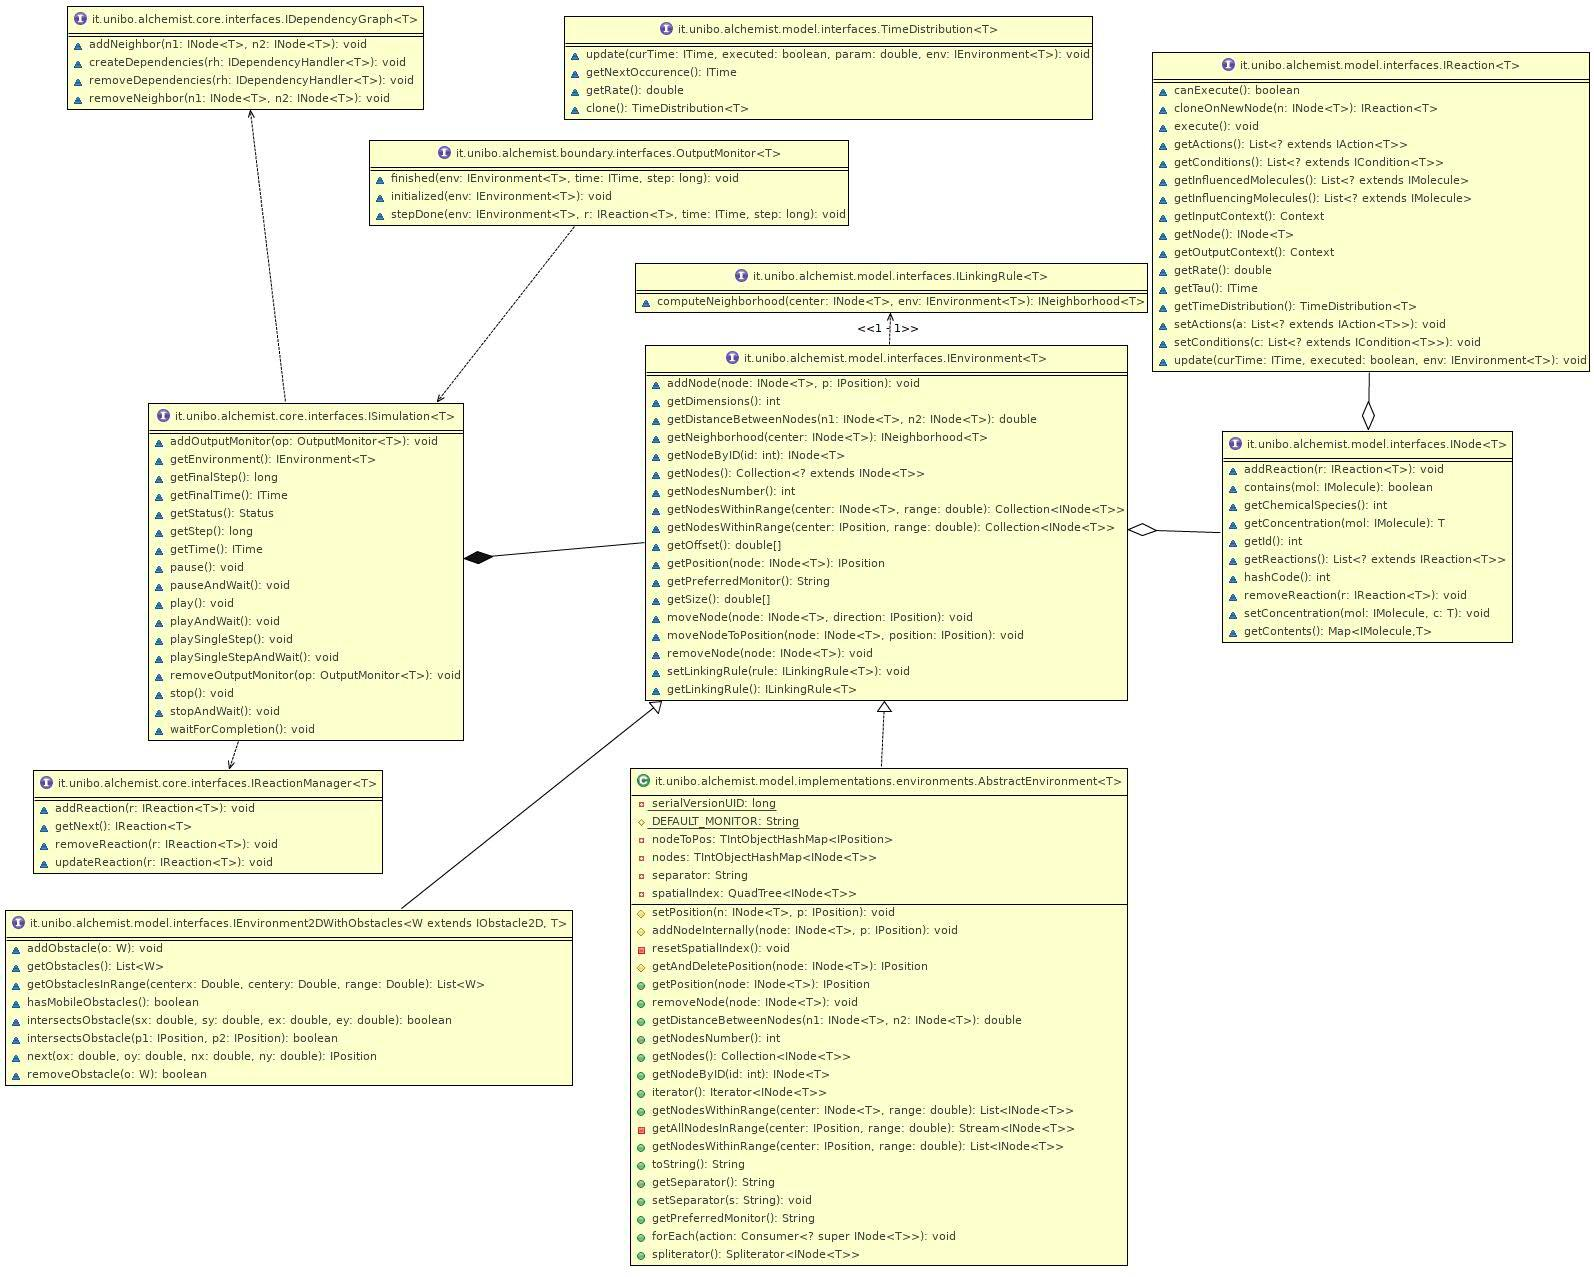
\includegraphics[width=\textwidth]{img/badarch}
	\caption{Schema UML mal fatto e con una pessima descrizione, che non aiuta a capire. Don't try this at home.}
	\label{img:badarch}
\end{figure}

%TODO: commentare questa parte del prof. quando avremo tutti finito di scrivere la nostra. -----------------  FINE -----------------------------------

% ----------------- ALESSANDRO PIOGGIA -----------------------------------------

\newpage

\subsection*{Alessandro Pioggia}
\textbf{Physical objects} \\ \\
Lo scopo iniziale del progetto è stato quello di creare delle vere e proprie entità di gioco(Players, Enemies, Obstacles, Items), che potessero popolare la mappa e interagire fra loro.
La mia parte richiedeva che io costruissi il core delle entità fisiche di gioco(oltre all'implementazione di alcune di esse), in modo da poter creare una struttura solida alla quale potessero fare riferimento i colleghi, sfruttando il principio della generalizzazione.

% ----------------- LEON BAIOCCHI -----------------------------------------

\newpage

\subsection*{Leon Baiocchi}

% ----------------- FEDERICO BRUNELLI -----------------------------------------

\newpage

\subsection*{Federico Brunelli}

% ----------------- LUCA RENGO -----------------------------------------

\newpage

\subsection*{Luca Rengo}

\textsf{\small La mia parte riguardava l'implementazione dei personaggi di gioco e dei diversi aspetti riguardanti la generazione della mappa e dei suoi componenti a livello di \emph{View}.}\\

\textsf{\small Mi competeva, inoltre, l'inizializzazione delle varie scene di gioco, dell'implementazione delle sprites, del salvataggio dei punteggi e delle statistiche completati dal giocatore.}\\ 
%della generazione della mappa a livello di \emph{View}.}\\

\subsubsection*{Characters}

\textsf{\small Per quanto concerne l'implementazione dei personaggi di gioco, ho sviluppato un'interfaccia \emph{Characters} che pone a tutte le figure l'implementazione di un contratto con le varie azioni comuni, i vari metodi che un personaggio può eseguire.}\\

\textsf{\small Questo è stato trattato dalle classi \emph{Player} ed \emph{Enemy} che contengono le proprietà e caratteristiche dei personaggi come la loro vita, il mana, il nome, le loro abilità e capacità come quella di muoversi e saltare.}\\

\textsf{\small Ho utilizzato poi un enum, \emph{EntityList}, per poter rappresentare diversi tipi di personaggi con diverse caratteristiche che ho settato nel metodo \emph{setPlayerType()} e \emph{setEnemyType()} delle rispettive classi. }\\

\textsf{\small Mi sono avvalso, inoltre, del pattern architetturale \textbf{Factory} per raccogliere le varie tipologie di \emph{Player} ed \emph{Enemy} attraverso l'interfaccia \emph{FactoryCharacters} e la sua implementazione \emph{FactoryCharactersImpl} per riorganizzare meglio i vari personaggi del gioco e rendere la loro creazione più chiara e semplice, evitando così di dover passare, ogni volta, un eccessivo numero di parametri da inizializzare.}

%TODO: immagine Model

\begin{figure}[h]
	\centering{} %TODO: aggiungere immagine UML
	%\includegraphics[width=\textwidth]{} 
	\caption{Schema UML del \emph{Model} relativo ai \emph{Characters}.}
	\label{img:uml_model_characters}
\end{figure}

\subsubsection*{Mappa di gioco} %TODO: approfondire la spiegazione. Descrivere le difficoltà incontrate e le soluzioni.

\textsf{\small Per quanto riguarda la \emph{Mappa} mi sono occupato degli aspetti della \emph{View}.}\\

\textsf{\small E' presente l'interfaccia \emph{GameView} che viene implementata dalla classe astratta \emph{AbstractScene} che ha il compito di rappresentare una generica scena del gioco, come la mappa o i crediti del gioco. Questa è ereditata dalla Classe \emph{MapScene} che implementa una specifica scena del gioco, ovvero quella della mappa, inizializzando tutte le sprites delle varie entità di gioco e generandole sullo schermo.}\\

\textsf{\small In \emph{MapScene} vengono generate le sprites dalle classi \emph{Platform}, \emph{Coin}, \emph{MainEnemy}, \emph{MainPlayer} con la sua animazione implementata in \emph{SpriteAnimation}.}\\

\textsf{\small Queste entità vengono posizionate in una precisa posizione in base alla locazione di un carattere in un array di stringhe che si trova nella classe \emph{LevelData}.} %TODO: sistemare, scrivere meglio.

\textsf{\small Ad ogni entità del gioco è associato un carattere che si trova nell'array di stringhe in \emph{LevelData}.}\\ %TODO: anche qui.

\textsf{\small Le classi \emph{Platform} e \emph{Coin} sono simili ed entrambe hanno un proprio enum per le proprie varie tipologie e utilizzano una ImageView per settare l'immagine, le proprietà e le posizioni sullo schermo.}\\

\textsf{\small \emph{MainEnemy} è una semplice ImageView statica mentre \emph{MainPlayer} è una ImageView dinamica, ovvero con un'animazione.}
\textsf{\small \emph{SpriteAnimation} è la classe che carica da \emph{MainPlayer} l'immagine e le sue caratteristiche (come width dell'immagine, height, ecc..) ed interpola le varie immagini della spritesheet del giocatore per creare la sua animazione che dura tot millisecondi.}\\

\textsf{\small  Quale sfondo della mappa da mostrare e la relativa piattaforma in tema e quale moneta vengono settate nella classe \emph{Map} che tiene traccia di questi elementi della View.}\\

%TODO: inserire UML della parte della mappa di gioco.

%TODO: parlare della Mappa (Map, MapScene, AbstractScene), del MainPlayer, SpriteAnimation, MainEnemy, Platform, Coin. LevelData

\subsubsection*{Salvataggio}

\textsf{\small Per quanto riguarda l'operazione di salvataggio delle statistiche di gioco, mi sono avvalso della classe \emph{Save} che crea un file di salvataggio in cui vengono contenuti il nome dei giocatori e i loro relativi punteggi.}\\

\textsf{\small Per fare questo, usufruisco di un \emph{BufferedWriter} per creare il file qualora questo non esista già. Altrimenti, mi limito ad aggiungere i dati in coda al file per evitare di eliminare ciò che era stato precedentemente memorizzato.}\\

\textsf{\small Poi mi avvalgo di un \emph{BufferedReader} per leggere dal file e memorizzare i dati e restituire un \emph{HashMap<String, Integer>} con il nome del player e il suo relativo punteggio.}\\

\textsf{\small Infine, ho un metodo per resettare il file e cancellare tutti i dati che erano stati immagazzinati.}\\

%TODO: aggiungere UML del salvataggio.

% -------------------------------- SVILUPPO -------------------------------------

\chapter{Sviluppo}
\section{Testing automatizzato}

Per il seguente progetto software è stato largamente sfruttato il testing automatizzato, dal momento che è stato scelto un approccio TDD(test-driven-development). Il nostro gruppo ha considerato opportuno testare prevalentemente la componente di logica(model) oltre ai vari controller.
Abbiamo inoltre attribuito importanza alla "pulizia" dei test, per garantire la loro manutenibilità, effettuando i seguenti accorgimenti : 

\begin{itemize}
	\item Utilizzo di una struttura fissa secondo il quale in primis si preparano i dati del test, successivamente si opera su di essi ed infine si controlla che i risultati siano quelli previsti. 
	\item Tentativo di mantenere i test indipendenti, in modo da poter individuare gli errori in modo preciso ed analitico.
	\item Dichiarazione dei metodi di test con nomi autoesplicativi, in modo da poter individuare lo scopo del test senza la necessità di inserire commenti ridondanti e voluminosi.
\end{itemize}

\subsection*{Alessandro Pioggia}

\begin{itemize}
	\item GameEntityTest;
	\item ObstacleTest;
	\item PickupItemTest;
	\item SpeedVector2DTest;
	\item Dimension2DTest;
\end{itemize}

\subsection*{Leon Baiocchi}

\begin{itemize}
	\item todo : scrivere le classi di test utilizzate
\end{itemize}

\subsection*{Federico Brunelli}

\begin{itemize}
	\item todo : scrivere le classi di test utilizzate
\end{itemize}

\subsection*{Luca Rengo}

\begin{itemize}
	\item \textsf{\small CharactersTest}
	\item \textsf{\small MapTest}
	\item \textsf{\small SaveTest}
\end{itemize}



\section{Metodologia di lavoro}

Nella prima fase di realizzazione del progetto ci siamo dedicati all'analisi, in cui abbiamo lavorato in maniera coordinata per definire la struttura e le funzionalità del progetto.
Successivamente siamo passati al design, in cui è stato deciso di creare uno scheletro in UML che descrivesse a grandi linee le entità principali necessarie per il funzionamento, definendo già le dipendenze fra esse. Il processo descritto ci ha permesso di definire una suddivisione del lavoro in 4 parti, in modo da garantire la prosecuzione del lavoro individuale con la fase di design dettagliato. \\
Per facilitare lo sviluppo abbiamo sfruttato un real-time-mantained UML, ovvero una repository in cui ciascun membro, una volta terminata una sessione di lavoro, aveva la premura di aggiornare uno schema UML, costruendo/modificando un diagramma delle classi che descrivesse il lavoro svolto. \\
Per quanto riguarda il DVCS abbiamo optato per l'utilizzo di git, in accordo con le nozioni apprese a lezione. La metodologia utilizzata è stata la seguente:

\begin{itemize}
	\item Sviluppo in feature-branches, ovvero branches in cui venivano realizzate singolarmente le feature dell'applicativo;
	\item Ognuno di noi aveva a disposizione un numero definito di branches indipendenti dagli altri;
	\item I feature-branches venivano poi confluiti nel main-branch.
\end{itemize}

\subsection*{Alessandro Pioggia}
Lavoro svolto : 
\begin{itemize}
	\item Realizzazione del menù principale con relativi reindirizzamenti.
	\item Creazione dello scheletro per l'implementazione delle entità di gioco fisiche, ovvero la creazione dell'interfaccia PhysicalObject la relativa implementazione;
	\item Implementazione di oggetti di gioco pickable (Item) e di ostacoli(Obstacles), realizzazione di sprites compresa;
	\item Creazione di commons, quali Dimension2D e SpeedVector2D;
	\item Creazione dello scheletro PhysicalObjectSprite, per la creazione delle sprite (aspetto di view);
	\item Gestione dei suoni.
\end{itemize}


\subsection*{Leon Baiocchi}

\begin{itemize}
	\item  todo : scrivere quello che si è fatto nel progetto.
\end{itemize}

\subsection*{Federico Brunelli}

\begin{itemize}
	\item  todo : scrivere quello che si è fatto nel progetto.
\end{itemize}

\subsection*{Luca Rengo}

\begin{itemize}
	\item  \textsf{\small Modellazione del \emph{giocatore} e dei \emph{nemici}.}
	\item \textsf{\small Composizione di una classe astratta per la formazione di una generica scena di gioco.}
	\item \textsf{\small Generazione della Mappa di gioco e delle relative entità dal punto di vista della \emph{View} come le \emph{piattaforme}, \emph{monete}, il \emph{giocatore} e i \emph{nemici}.}
	\item \textsf{\small Implementazione dell'animazione del player.}
	\item \textsf{\small Creazione di una classe per il salvataggio dei dati e delle statistiche di gioco.}
\end{itemize}

\section{Note di sviluppo}

\subsection*{Alessandro}

\begin{itemize}
	\item  \textbf{\textit{JavaFx}} : utilizzato per la realizzazione del menù;
	\item \textbf{\textit{Optionals}} : per evitare di ritornare valori null;
	\item \textbf{\textit{Apache library}} : libreria che ho importato per l'utilizzo delle classi Pair preimplementate;
	\item \textbf{\textit{Gradle}} : strumento che ho utilizzato per importare le varie componenti di javafx;
	\item \textbf{\textit{Reflection}} : utilizzata per la creazione delle statistiche, perchè richiesta da javafx;
	\item \textbf{\textit{JUnit}} : utilizzata per il testing;
	\item \textbf{\textit{Streams e lambda}} : utilizzate dove possibile, per migliorare la leggibilità e l'efficienza.
\end{itemize}

\subsection*{Leon Baiocchi}

\begin{itemize}
	\item  todo : scrivere quello che si è fatto nel progetto.
\end{itemize}

\subsection*{Federico Brunelli}

\begin{itemize}
	\item  todo : scrivere quello che si è fatto nel progetto.
\end{itemize}

\subsection*{Luca Rengo}

\begin{itemize}
	\item \textsf{\small \textbf{JavaFX}: sfruttato per la realizzazione della mappa e delle sue componenti.}
	\item \textsf{\small \textbf{Factory}: adoperata per raggruppare le mie classi ed instanziarle più facilmente.}
	\item \textsf{\small \textbf{JUnit}: beneficiata per l'esaminazione delle parti di codice create.}
	\item \textsf{\small \textbf{Lambda}: utilizzate per semplificare alcune parti del programma.}
	\item \textsf{\small \textbf{Gradle}: impiegato per importare i vari moduli di JavaFX, JUnit e le varie dipendenze e per tenere il progetto ben organizzato.}
\end{itemize}

% ------------------------ COMMENTI FINALI---------------------------------------

\chapter{Commenti finali}

In quest'ultimo capitolo si tirano le somme del lavoro svolto e si delineano eventuali sviluppi
futuri.

\textit{Nessuna delle informazioni incluse in questo capitolo verrà utilizzata per formulare la valutazione finale}, a meno che non sia assente o manchino delle sezioni obbligatorie.
%
Al fine di evitare pregiudizi involontari, l'intero capitolo verrà letto dai docenti solo dopo aver formulato la valutazione.

\section{Autovalutazione e lavori futuri}

\textbf{È richiesta una sezione per ciascun membro del gruppo, obbligatoriamente}.
%
Ciascuno dovrà autovalutare il proprio lavoro, elencando i punti di forza e di debolezza in quanto prodotto.
Si dovrà anche cercare di descrivere \emph{in modo quanto più obiettivo possibile} il proprio ruolo all'interno del gruppo.
Si ricorda, a tal proposito, che ciascuno studente è responsabile solo della propria sezione: non è un problema se ci sono opinioni contrastanti, a patto che rispecchino effettivamente l'opinione di chi le scrive.
Nel caso in cui si pensasse di portare avanti il progetto, ad esempio perché effettivamente impiegato, o perché sufficientemente ben riuscito da poter esser usato come dimostrazione di esser capaci progettisti, si descriva brevemente verso che direzione portarlo.

\section{Difficoltà incontrate e commenti per i docenti}

Questa sezione, \textbf{opzionale}, può essere utilizzata per segnalare ai docenti eventuali problemi o difficoltà incontrate nel corso o nello svolgimento del progetto, può essere vista come una seconda possibilità di valutare il corso (dopo quella offerta dalle rilevazioni della didattica) avendo anche conoscenza delle modalità e delle difficoltà collegate all'esame, cosa impossibile da fare usando le valutazioni in aula per ovvie ragioni.
%
È possibile che alcuni dei commenti forniti vengano utilizzati per migliorare il corso in futuro: sebbene non andrà a vostro beneficio, potreste fare un favore ai vostri futuri colleghi.
%
Ovviamente \textit{il contenuto della sezione non impatterà il voto finale}.

% -------------------------- APPENDICI ------------------------------------------

\appendix
\chapter{Guida utente}

\subsection{Modalità d'uso}

\textsf{\small Per avviare l'applicazione occorre eseguire il comando \emph{./gradlew run}.} \\

\subsection{Requisiti}

\begin{itemize}
	\item \textsf{\small JDK 11+}
	\item \textsf{\small Gradle 8+}
\end{itemize}

\subsection{Comandi del gioco}

\begin{itemize}
	\item \textsf{\small freccia su : saltare}
	\item \textsf{\small freccia destra : andare a destra}
	\item \textsf{\small freccia sinistra : andare a sinistra}
	\item \textsf{\small spazio : sparare}
\end{itemize}

\subsection{Impostazioni di Gioco}

\textsf{\small Attraverso il menù di gioco è possibile modificare le impostazioni: } \\

\begin{itemize}
	\item \textsf{\small Risoluzione}
	\item \textsf{\small Livello di difficoltà}
	\item \textsf{\small Volume}
	\item \textsf{\small Lingua:}
	\begin{itemize}
		\item \textsf{\small Inglese}
		\item \textsf{\small Italiano}
		\item \textsf{\small Spagnolo}
		\item \textsf{\small Tedesco}
		\item \textsf{\small Polacco}
		\item \textsf{\small Russo}
		\item \textsf{\small Arabo Standard Moderno}
		\item \textsf{\small Francese}
		\item \textsf{\small Giapponese}
	\end{itemize}
\end{itemize}

\chapter{Esercitazioni di laboratorio}

\textsf{\small Qui di seguito, i links di alcuni esercizi che abbiamo svolto:} \\

\section*{Esempio}

\subsection{Alessandro Pioggia}

\begin{itemize}
	\item Laboratorio 04: \url{https://virtuale.unibo.it/mod/forum/discuss.php?d=62685#p101507}
	\item Laboratorio 05: \url{https://virtuale.unibo.it/mod/forum/discuss.php?d=62684#p101217}
	\item Laboratorio 06: \url{https://virtuale.unibo.it/mod/forum/discuss.php?d=62579#p100880}
	\item Laboratorio 07: \url{https://virtuale.unibo.it/mod/forum/discuss.php?d=62582#p100893}
	\item Laboratorio 08: \url{https://virtuale.unibo.it/mod/forum/discuss.php?d=63865#p107314}
	\item Laboratorio 09: \url{https://virtuale.unibo.it/mod/forum/discuss.php?d=64639#p103992}
	\item Laboratorio 10: \url{https://virtuale.unibo.it/mod/forum/discuss.php?d=66753#p106887}
\end{itemize}

\subsection{Leon Baiocchi}

\begin{itemize}
	\item Laboratorio 04: \url{https://virtuale.unibo.it/mod/forum/discuss.php?d=62685#p101274}
	\item Laboratorio 05: \url{https://virtuale.unibo.it/mod/forum/discuss.php?d=62684#p101286}
	\item Laboratorio 06: \url{https://virtuale.unibo.it/mod/forum/discuss.php?d=62579#p100978}
	\item Laboratorio 07: \url{https://virtuale.unibo.it/mod/forum/discuss.php?d=62582#p101496}
	\item Laboratorio 08: \url{https://virtuale.unibo.it/mod/forum/discuss.php?d=63865#p103119}
	\item Laboratorio 09: \url{https://virtuale.unibo.it/mod/forum/discuss.php?d=64639#p104957}
	\item Laboratorio 10: \url{https://virtuale.unibo.it/mod/forum/discuss.php?d=66753#p106591}
\end{itemize}


\bibliographystyle{alpha}
\bibliography{13-template}

\end{document}
